% id: 0201
% book: RPM 중3-2 수학 · 02 삼각비의 활용
% section: 유형 08 삼각형의 넓이 – 예각이 주어진 경우
% figure: crop:fig-0201.png
% answer: $45^\circ$
% answer_source: 답지
% variant_level: 0 (원본 전사)
% 이 파일은 build.mjs 가 items.json 에서 만든다. 고칠 때는 items.json 을 고친다.
\noindent\begin{minipage}[t]{0.58\linewidth}\vspace{0pt}\raggedright 오른쪽 그림과 같이 $\seg{AB}=6$, $\seg{BC}=10$인 $\triangle\pt{ABC}$의 넓이가 $15\sqrt{2}$일 때, $\angle\pt{B}$의 크기를 구하시오. \dmcondfill{$0^\circ<\angle\pt{B}<90^\circ$}{}\end{minipage}\hfill\begin{minipage}[t]{0.4\linewidth}\vspace{0pt}\centering \setlength{\dmfigw}{93.3pt}\ifdim\dmfigw>\linewidth\setlength{\dmfigw}{\linewidth}\fi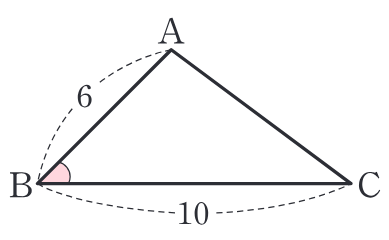
\includegraphics[width=\dmfigw]{figures/fig-0201.png}\end{minipage}\par
